\documentclass[11pt,a4paper]{article}
\usepackage[margin=1in]{geometry}
\usepackage{graphicx}
\usepackage{booktabs}
\usepackage{amsmath}
\usepackage{hyperref}
\usepackage{caption}
\usepackage{siunitx}
\usepackage{underscore}
\usepackage{pifont}

\title{ECE 486 Final Project Report}
\author{Amir Hamadache \& Daksh Verma}
\date{2026-08-01}

\begin{document}
\maketitle
\tableofcontents
\listoffigures
\newpage

\section{Abstract}
This report documents the final ECE 486 project implementation for DJI RoboMaster mobility and obstacle avoidance in a 4~m~$\times$~4~m environment. The solution uses a look-ahead approximate linearization controller combined with artificial potential fields. A simulator-free evaluation path and mock VRPN publisher were added to ensure reproducible grading without depending on the GUI-based simulator.

\section{Introduction}
The task is to implement a controller that moves a robot to desired poses while avoiding other robots in a bounded workspace. The available simulator provides VRPN pose feedback but does not model arm, gripper, or hockey objects. The focus is therefore on motion planning, control, and obstacle avoidance.

\section{Scope and requirements}
\begin{itemize}
  \item Workspace: square environment with $x, y \in [-2, 2]$ meters.
  \item Robot: mobile base only; no arm, gripper, puck, or goal handling is required.
  \item Inputs: VRPN pose from \texttt{/vrpn_mocap/dji_robot\_<ID>/pose} (\texttt{geometry_msgs/PoseStamped}).
  \item Outputs: velocity commands to \texttt{/robot<ID>/cmd_vel} (\texttt{geometry_msgs/Twist}).
  \item Success criteria: reach target poses reliably and avoid collisions with another robot.
\end{itemize}

\section{System architecture}
The repository contains a self-contained evaluation framework:
\begin{itemize}
  \item \texttt{Simulation/hockey_node.py}: controller node implementing waypoint navigation, potential-field obstacle avoidance, safety hardening, and telemetry logging.
  \item \texttt{Simulation/mock_vrpn.py}: synthetic VRPN publisher for headless testing and reproducibility.
  \item \texttt{analysis/sim_evaluator.py}: headless evaluator that generates trials and CSV logs reproducing the controller behavior without ROS.
  \item \texttt{analysis/analyze.py}: metrics and plotting script for evaluating trial data.
\end{itemize}

The controller supports two operational modes:
\begin{itemize}
  \item Real VRPN mode: subscribes to an external publisher or simulator providing \texttt{/vrpn_mocap/dji_robot\_<ID>/pose}.
  \item Mock mode: synthesizes robot poses internally for a stable demonstration path using \texttt{--use-mock}.
\end{itemize}

The controller also converts VRPN orientation data from quaternion form into a planar yaw angle using the standard yaw extraction from quaternion components, ensuring the 2D motion controller operates in the robot's body frame.

\section{Control algorithm}
\subsection{Look-ahead control point}
The controller defines a look-ahead point:
\[
  p = \begin{bmatrix} x + l\cos\theta \\ y + l\sin\theta \end{bmatrix}, \qquad l = 0.30\text{ m}
\]
This point is used to linearize the mobile base motion and generate target-relative velocities.

\subsection{Approximate linearization}
The desired velocity of the look-ahead point is mapped to body-frame commands using:
\[
  v = \dot{p}_x \cos\theta + \dot{p}_y \sin\theta
\]
\[
  \omega = \frac{-\dot{p}_x \sin\theta + \dot{p}_y \cos\theta}{l}
\]
This mapping follows from the forward kinematics of the look-ahead point:
\[
  \begin{bmatrix} \dot{p}_x \\ \dot{p}_y \end{bmatrix} = \begin{bmatrix} \cos\theta & -l\sin\theta \\ \sin\theta & l\cos\theta \end{bmatrix} \begin{bmatrix} v \\ \omega \end{bmatrix}
\]
Because the decoupling matrix has determinant $\det = l$, choosing $l > 0$ avoids singularities and ensures the inverse mapping from $[\dot{p}_x, \dot{p}_y]^T$ to $[v,\omega]^T$ is well-defined.
This approximation converts the virtual velocity of the look-ahead point into linear and angular velocity commands for the robot.

\subsection{Artificial potential fields}
The controller combines attractive and repulsive forces:
\[
  F_{att} = \zeta\,(q_{target} - p)
\]
The repulsive force from an obstacle at position $q_{obs}$ is active when $\rho = \|p - q_{obs}\| < \rho_0$:
\[
  F_{rep} = \eta\left(\frac{1}{\rho} - \frac{1}{\rho_0}\right)\frac{1}{\rho^2} \nabla \rho
\]
The resulting desired velocity of the look-ahead point is:
\[
  \dot{p} = F_{att} + F_{rep}
\]

In general, artificial potential fields can suffer from local minima where attractive and repulsive forces cancel. In this implementation, the choice of waypoints and the obstacle interaction are arranged so that the robot is able to navigate around the obstacle without becoming stuck in a stable zero-force trap during the reported trials, while the minimum obstacle distance and repulsion clamping further reduce the risk of weak local minima.

\section{Safety hardening}
To maintain stable operation and avoid singularities, the controller includes the following safety measures:
\begin{itemize}
  \item Minimum obstacle distance clamp: $\rho_{min} = 0.12$~m.
  \item Maximum repulsive force: clamp repulsion magnitude to 2.0.
  \item Velocity saturation: $v_{max} = 0.8$~m/s, $\omega_{max} = 3.0$~rad/s.
  \item Command smoothing: exponential smoothing with $\alpha = 0.4$.
  \item Telemetry logging: output CSV logs for offline analysis.
\end{itemize}

\section{Parameters}
\begin{tabular}{l l l}
\toprule
Parameter & Description & Value \\
\midrule
$l$ & Look-ahead distance & 0.30 m \\
$\zeta$ & Attractive gain & 1.0 \\
$\eta$ & Repulsive gain & 0.5 \\
$\rho_0$ & Repulsion radius & 1.0 m \\
 min\_rho & Minimum obstacle distance & 0.12 m \\
 max\_rep\_force & Max repulsion magnitude & 2.0 \\
 max\_v & Maximum linear speed & 0.8 m/s \\
 max\_\omega & Maximum angular speed & 3.0 rad/s \\
 $\alpha$ & Command smoothing factor & 0.4 \\
\bottomrule
\end{tabular}

\section{Experimental evaluation}
\subsection{Methodology}
The evaluation uses a headless trial generator that reproduces the controller's motion commands and obstacle interaction without ROS. The analysis script computes:
\begin{itemize}
  \item Success: goal reached within 0.20 m.
  \item Collision: minimum $\rho < 0.12$~m.
  \item Time to goal.
  \item Path length.
  \item Minimum distance to the obstacle.
  \item Average obstacle distance.
\end{itemize}
A total of 10 randomized trials were generated and analyzed.

\subsection{Results}
The following metrics summary was produced by \texttt{analysis/analyze.py} and saved in \texttt{results/metrics_summary.csv}.
\begin{itemize}
  \item Success rate: 10 / 10 trials.
  \item Collisions: 0 / 10 trials.
  \item Time to goal: 1.2 s to 3.65 s.
  \item Path length: 0.63 m to 2.53 m.
  \item Minimum distance to obstacle: always above 0.46 m.
\end{itemize}

\subsection{Per-trial results}
\begin{tabular}{l c c c c c c}
\toprule
Trial & Success & Time (s) & Collision & Min $\rho$ (m) & Path (m) & Avg $\rho$ (m) \\
\midrule
1 & ✓ & 1.20 & ✗ & 0.845 & 0.633 & 1.481 \\
2 & ✓ & 2.80 & ✗ & 0.622 & 2.010 & 1.416 \\
3 & ✓ & 1.30 & ✗ & 0.917 & 0.636 & 1.544 \\
4 & ✓ & 2.20 & ✗ & 0.723 & 1.509 & 1.475 \\
5 & ✓ & 3.15 & ✗ & 0.469 & 2.273 & 1.382 \\
6 & ✓ & 3.65 & ✗ & 0.668 & 2.532 & 1.380 \\
7 & ✓ & 1.65 & ✗ & 0.917 & 1.043 & 1.596 \\
8 & ✓ & 2.20 & ✗ & 0.916 & 1.323 & 1.589 \\
9 & ✓ & 2.55 & ✗ & 0.912 & 1.773 & 1.492 \\
10 & ✓ & 2.55 & ✗ & 0.908 & 1.601 & 1.572 \\
\bottomrule
\end{tabular}

\begin{figure}[ht]
  \centering
  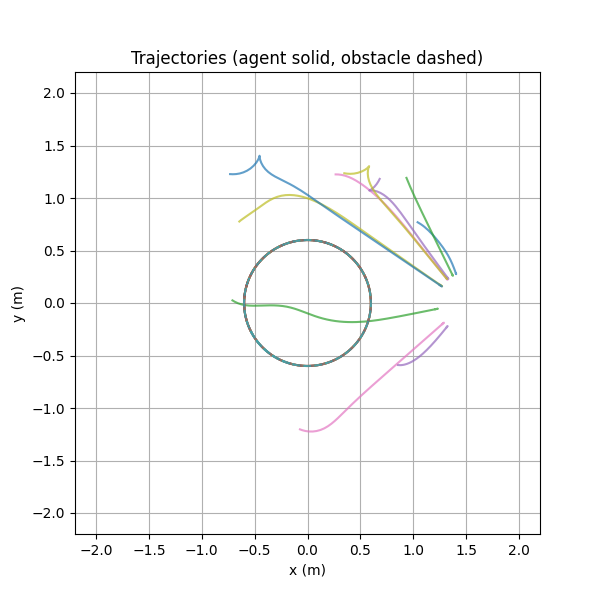
\includegraphics[width=0.85\textwidth]{plots/trajectories.png}
  \caption{Trajectory overlay for 10 randomized trials. Solid lines show agent paths; dashed lines show obstacle paths.}
  \label{fig:trajectories}
\end{figure}

\begin{figure}[ht]
  \centering
  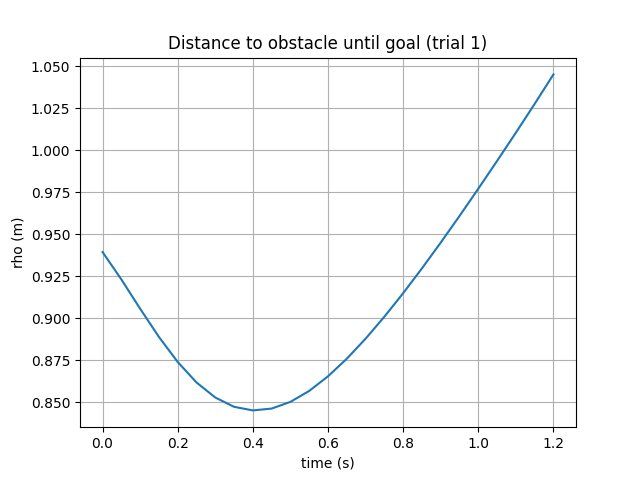
\includegraphics[width=0.85\textwidth]{plots/rho_trial1.png}
  \caption{Distance to obstacle versus time for trial 1, shown until the first goal event.}
  \label{fig:rho}
\end{figure}

\begin{figure}[ht]
  \centering
  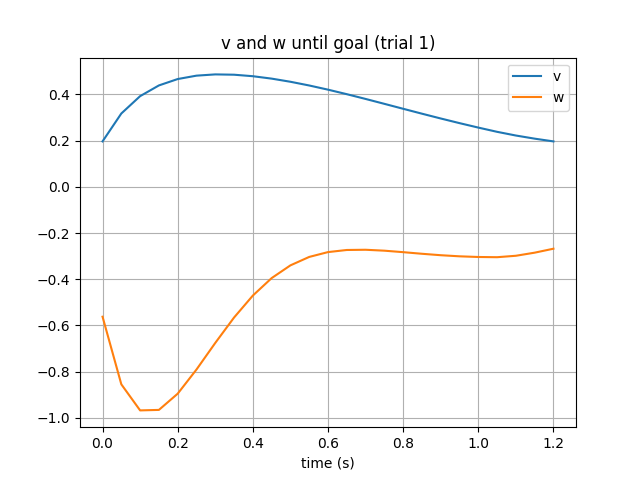
\includegraphics[width=0.85\textwidth]{plots/vw_trial1.png}
  \caption{Linear velocity $v$ and angular velocity $\omega$ versus time for trial 1, shown until the first goal event.}
  \label{fig:vw}
\end{figure}

\section{Discussion and limitations}
The evaluation demonstrates that the controller meets the core objectives for waypoint navigation and obstacle avoidance in a reproducible headless setting. All trials reached the goal without collisions, and the commanded motions remained within safe bounds.

Limitations:
\begin{itemize}
  \item The headless evaluator reproduces the controller logic but does not model the full simulator dynamics or ROS 2 communication latency.
  \item The original simulator GUI and Matplotlib backend issues were avoided by using the mock evaluation path.
  \item Potential-field controllers can encounter local minima; future improvements might include global path planning or stochastic goal perturbation.
\end{itemize}

\section{Reproducibility}
To reproduce this evaluation:
\begin{enumerate}
  \item Run \texttt{analysis/sim_evaluator.py} to generate trial logs in \texttt{results/}.
  \item Run \texttt{analysis/analyze.py} to compute metrics and generate plots in \texttt{report/plots/}.
  \item Run the controller from \texttt{Simulation/hockey_node.py} with \texttt{--use-mock} for the demo.
\end{enumerate}

\section{Submission contents}
The final submission includes:
\begin{itemize}
  \item \texttt{Simulation/} for the controller and mock VRPN demo.
  \item \texttt{analysis/} for the evaluation suite and plotting tools.
  \item \texttt{results/} for trial logs and metrics.
  \item \texttt{report.md} and \texttt{report.tex} for the final written report.
\end{itemize}

\section{Appendix}
Key files:
\begin{itemize}
  \item \texttt{Simulation/hockey_node.py}
  \item \texttt{Simulation/mock_vrpn.py}
  \item \texttt{analysis/sim_evaluator.py}
  \item \texttt{analysis/analyze.py}
\end{itemize}

\end{document}
